\section{Data Analysis}
	\subsection{CRISP-DM}
	\label{sec:datamodeling}
	\begin{figure}[h]
		\centering
		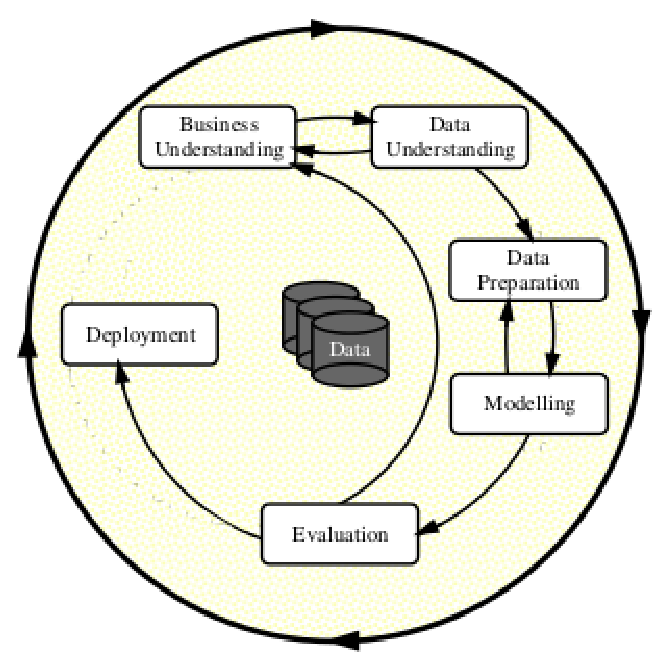
\includegraphics[scale=0.75]{crispdm.eps}
					
		\caption{CRISP-DM \cite{wirth2000crisp} cycle}
		\label{fig:crispdm}

	\end{figure}
	This section has some theory, to get a view of the big picture. Cross Industry Standard Process for Data Mining \cite{wirth2000crisp} is invented out of necessity for better planning, documentation and communication for Data Mining projects. It is divided in multiple phases, as seen in Figure~\ref{fig:crispdm}. The business understanding phase is to describe the urge and the goal of the project, see Section~\ref{seq:motivation}. The data understanding phase is to learn about the data, what is the source and how it is computed. In Section~\ref{sec:sensorsystems},~\ref{sec:datadescription} and ~\ref{sec:bvsb} the sensors systems are described, how they are used and what the data is. Normally the data is already collected, but this project needs another phase. The data collection phase is described in Section~\ref{sec:datacollection}. The next phase is the data preparation phase. In this project it exists out of two parts. The first part is about preprocessing to compute the dataset, as seen in Section~\ref{sec:preprocessing}. The dataset can be used by the Liacs Data Mining Group for further research. The second part is the feature extraction section, which describes the computing of the new dataset, seen in Section~\ref{sec:feature}. 
	A model is a generalised representation of the data. An algorithm tries to make relations between attributes. There are three reasons to make such a model:
	\begin{enumerate}
		\item Prediction. A bank give loans to clients and they will try to choose the best interest rate, such that the client will accept the interest rate, can pay the interest rate and the loan back over time and the bank will make a profit. Based on data from old clients a model can be made and the probability (prediction) of a client getting problems with paying the intereset rate can be calculated. Based on this information the high of the loan and the interest rate can be determined \cite{credit}. Another example is predicting the age of a Twitter user \cite{tweetgenie}.		
		\item Insight. After analyzing the correlation between products bought together in a supermarket, management decided to place diapers and beer close together. More customers who bought the diapers were tempted to buy the beer just by seeing it, which resulted in more impulsive sales \cite{beer}.
		\item Classification. Email spam (unwanted email) filters are using classification to determine if an email is spam or ham (not spam). Based on the previous received emails with their associated label spam or ham, a model can be made to predict the class of a new received email. 
	\end{enumerate}
	Models need to be trained by a dataset. The bigger the dataset, the better the model, because the chance is higher the set will represent all possible data. The better the model, the better the relations between the attributes are expressed. Section~\ref{sec:classification} makes a decision tree to make it possible to classify the location of a instance based on the data of the BioHarness. Section~\ref{sec:correlations} analyzes the correlations between features. The evaluation phase the conclusions are made and will be decided what to do next. The deployment is the implementation to achieve the goal. This could be a new piece of software for bank employees or a new price for a product. In this project there is no deployment.

	\subsection{Classification}
	\label{sec:classification}
	In this section a model is built of the locations based on the data of the BioHarness and the OpenBeacon. The dataset from Section~\ref{sec:rawdataset}  is used, with two alterations. The nights are removed, because the BioHarness does not measure in the night. The rows with missing values are also removed. This gives us a dataset with nearly 585000 instances or rows. WeKa \cite{weka} is a software program with a lot of data mining algorithms included and is used to make the model. The used algorithm is J48 and is an implementation of the C4.5 \cite{quinlan1993c4} decision tree algorithm. 66\% is used as training set and 34\% as validation set. Leafes with less than 10000 instances are removed. This will result in a pruned tree and will prevent overfitting. As a result of the actions to prevent overfitting, the percentage correctly classified instances is only 70\%, despite the large amount of instances. Only the locations ``out'', ``bedroom'' and ``rest of the house'' are classified, because those are most visited as seen in Figure~\ref{fig:histogram}. The tree is still big with 35 leafes. In this setup the data of the BioHarness could only explain some regular visited locations. It could be improved by stratifying sampling. This means the same amount of instances are used of every location, but this will make the model less realistic. It could also be improved by using more specific locations, for instead of the general ``out of the house'' location. I could do all kind of activies out of the house, which also applies for rest of the locations. An other solution could be the use of a lower sampling frequency, like $\frac{1}{60}$ \SI{}{\hertz} (every minute) instead of \SI{1}{\hertz} (every second). See Figure~\ref{fig:classtree} for the decision tree. \\
	The model is built again, because not all the locations showed up in the desicion tree. The difference is this time the three will be pruned less. Leafes with less than 1000 instances are removed. This results in a larger tree (114 leafes), a higher percentage correctly classified instances (74\%) and more locations showed up (living.room). Figure~\ref{fig:confusionmatrix} shows the confusion matrix of the second model. The best model possible has only numbers on the diagonal (the green circles), because those are the correctly classified instances. The blue circles shows there are many instances classified as \emph{out}, but they were actually \emph{rest.of.the.house} and \emph{bedroom}. The numbers in the red circles were classified as \emph{bedroom}, but were actually \emph{out} and \emph{rest.of.the.house}. These three locations are confused with each other, but that is logic because those are the major visited places. If you look at the horizontal numbers of \emph{out} you see the number at the diagonaal (from top left to right bottom) is the biggest. This also true for the horizontal numbers of \emph{bedroom}, but it is not true for \emph{rest.of.the.house} and \emph{living.room}. Most of the instances are predicted wrong. There are also zero values on the diagonal. This is because the locations \emph{dining.room}, \emph{toilet.ground.floor}, \emph{kitchen}, \emph{hall.first.floor}, \emph{toilet.first.floor} are a small percentage of the dataset and do not show up in the decision tree.

			\begin{figure}[h]
				\centering
					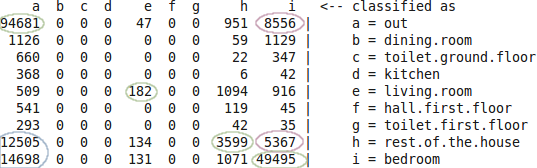
\includegraphics[scale=0.7]{confusion.png}
					
				\caption{Confusion Matrix.}
				\label{fig:confusionmatrix}

			\end{figure}


	
	\begin{figure}[h]
		\label{fig:classtree}	
		\centering
		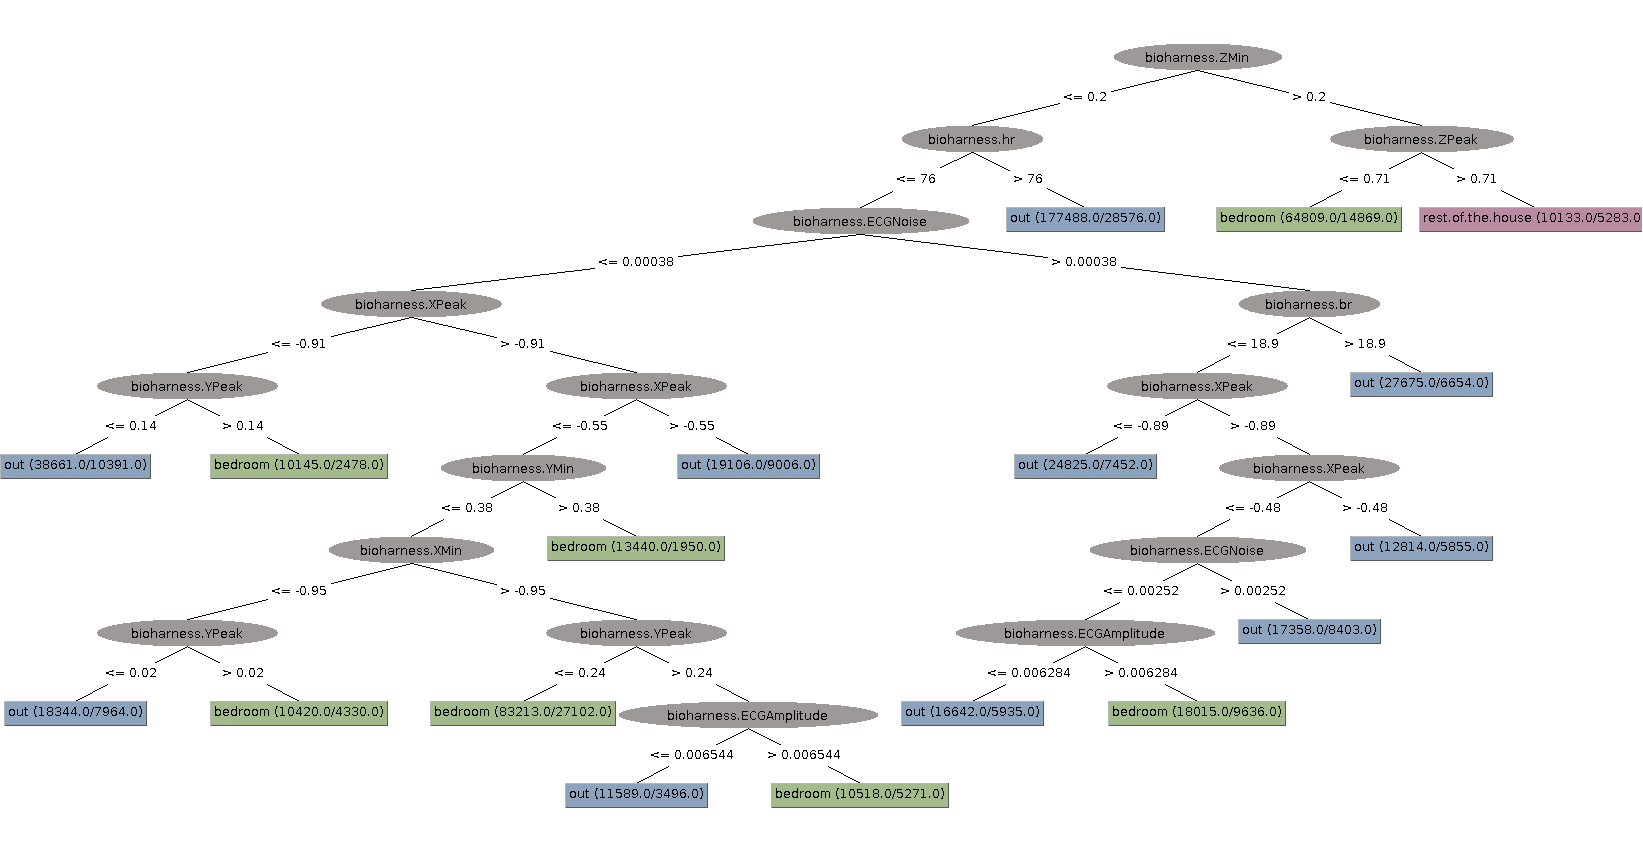
\includegraphics[scale=0.40, angle=90]{tree/edited.png}
		\caption{A decision tree of the first model.}
	\end{figure}


	\iffalse
	\subsection{WeKa}
	- What is WeKa. java implementation for a lot of data mining algorithms.
	- M5p, Quinlan's M5
	- linear regression
	- neural network
	- results 

	avgHr vs hr100+
	out vs bedroom
	out vs hr120-140
	dining.room - kitchen

	inbed vs avgNoise: hoe later naar bed -> hoe minder geluid?, doordat je waarschijnlijk niet aanwezig bent in de kamer.
	outbed vs stageA: later naar bed, vaker away, later opstaan.
	outbed vs inbed: correlatie is 0.21. 

	light sleep neemt toe naarmate ik later naar bed ga, maar deep sleep ook. Val dus sneller in slaap. 
	Sleep efficiency neemt toe als ik latar naar bed ga. (r=0.5) Later opstaan zorgt juist voor het tegenovergestelde.
	later naar bed gaan dan gisteren resulteert ook in lagere sleep efficiency
	outbed vs inbed: r = 0.49
	Sta ik later naar bed, of later uit bed dan gisteren, gaat de efficiency omlaag 
	target

	\fi
	\subsection{Correlations}
	\label{sec:correlations}
	In Table \ref{tab:cor}, 28 correlations are listed. These correlations are based on the dataset produced in Section~\ref{sec:feature}. Analyzing the results gives some trivial conclusions, but also interesting ones. \#3 says when I wake up later, the difference between the previous wake up is greater. The higher the correlations the more consistent the sleep rythm. \#6 says, the later I go to bed, the more I am away from my bed. \#11 is also trivial. \#1 and \#4 are more interesting, because it means when I diverge from my normal sleep rythm, I will sleep less efficient. Going later to bed and waking up later will result\footnote{``Will result'' is not precisely true. Correlation does not mean causality, but in this paragraph the causalities are assumed.}  in less REM sleep and it will not be at the expense of deep sleep. As a matter of fact, the correlation is positive, it will result in a bit more deep and light sleep. Going later to bed will result in less time awake in bed, but sleeping longer in the morning will result in more awake time. \#18 is also an interesting correlation, but the resting heart rate is relative constant, so it does not need to mean anything. A high heart rate will result in a less efficient sleep, based on \#20 and \#27, but based on \#21 and \#24 it will result in more deep sleep. Most trivial correlation is \#28, because stageW is part of the formula to calculate the sleep efficiency.
		

	\clearpage
	\begin{table}
		\centering
		\newcounter{rownum}
		\setcounter{rownum}{0}
		\newcommand\rownumber{\stepcounter{rownum}\arabic{rownum}}
	\begin{tabular}{| c | l | l | l |}
		\hline
		\# & Feature A & Feature B & Correlation \\ \hline
		\rownumber & outbed.difference\tablefootnote{The amount of minutes woke up later than the previous day} & sleep.efficiency\tablefootnote{Relative time slept in bed} & -0.51 \\
		\rownumber & outbed\tablefootnote{Amount of minutes woke up after 08:00 am} & inbed.difference & 0.33 \\
		\rownumber & outbed & outbed.difference & 0.54 \\
		\rownumber & inbed.difference & sleep.efficiency & -0.14 \\
		\rownumber & inbed\tablefootnote{Amount of minutes going to bed after 22:00 pm} & outbed & 0.21 \\ 
		\rownumber & inbed & stageA\tablefootnote{Away} & 0.50 \\
		\rownumber & inbed & stageW\tablefootnote{Wake} & -0.53 \\
		\rownumber & inbed & stageD\tablefootnote{Deep sleep} & 0.10 \\
		\rownumber & inbed & stageL\tablefootnote{Light sleep} & 0.09 \\
		\rownumber & inbed & stageR\tablefootnote{REM sleep} & -0.40 \\
		\rownumber & outbed & stageA & -0.74 \\    
		\rownumber & outbed & stageW & 0.13 \\    
		\rownumber & outbed & stageL & 0.07 \\
		\rownumber & outbed & stageD & 0.03 \\
		\rownumber & outbed & stageR & -0.67 \\
		\rownumber & hr100+ & resting.heartrate & 0.28 \\
		\rownumber & stress.percent & resting.heartrate & -0.35 \\
		\rownumber & out\tablefootnote{Out of the house} & resting.heartrate & 0.65 \\
		\rownumber & stageD & resting.heartrate & -0.15 \\
		\rownumber & hr140+ & sleep.efficiency & -0.59 \\
		\rownumber & hr100+ & stageD & 0.25 \\
		\rownumber & hr100+ & stageL & -0.13 \\
		\rownumber & hr100+ & stageR & -0.41 \\
		\rownumber & avgHR & stageD & 0.32 \\
		\rownumber & avgHR & stageL & -0.17 \\
		\rownumber & avgHR & stageR & -0.46 \\
		\rownumber & avgHR & sleep.efficiency & -0.39 \\
		\rownumber & stageW & sleep.efficiency & -0.99 \\

		\hline
	\end{tabular}
	\caption{A few correlations between different features}
	\label{tab:cor}
	\end{table}
	

	\iffalse

	Business understanding: formulate a goal, what to improve, section 1.2 / 1.3
	Data understanding, What are the systems measuring : Section 2.
	Normally data is already collected, in this project not. So an extra step.
	Data preparation is getting from the raw data to the training set, but in this project there are to steps to produce it.
	First from the raw to the dataset. This dataset can is provided and can be used by the liacs data mining group.
	from dataset to trainingset, in feature extractin section



	Derivate a dataset, use WeKa for modeling, find patterns.

	
	model, A way to describe the data. Generalization.
	prediction, classification, understanding the model.
	- linear regression
	- nearal network
	Now the modeling part.

	Next is the evaluation, which conclusions could be made.

	At least the deployment, implementation of the conclusions. To reach the goal and improvement. 
	\fi
